% DONE: too wordy
%\section{Consistent Parameter Estimation in Directed Models}
\section{Directed models and exclusive views}
\label{sec:directed}

%\todo{we are using clique to refer to only hidden cliques; be explicit about using "hidden"}

% DONE: need more setup of what the goal is
%The tensor factorization method attacks the heart of the non-convexity
  %in latent variable models.
  In this section, we will develop a consistent parameter estimate for a class of directed graphical models.
  In general directed models, the conditional moments $\mOpp{v}{i} \eqdef \Pr(x_v \mid h_i)$
which we were able to recover from {\TensorFactorize}, are not the underlying parameters.
  %Once we recover the conditional moments $\mOpp{v}{j} \eqdef \Pr(x_v
  %| h_j)$ for some $v, j$, we present a systematic approach to learn the
  %conditional probability tables for every clique for a class of directed
  %graphical models.
  Let us first consider an example (Section~\ref{sec:directedExample});
  Section~\ref{sec:directedGeneral} will describe the algorithm in full generality.
For ease of exposition we make the following simplifications to our presentation:
(i) we describe our algorithm entirely in the context of directed
  graphical models, though it generalizes to undirected models;
(ii) we derive our algorithm assuming infinite data; in \sectionref{sampleComplexity} we 
  describe error bounds for the finite sample regime; and
(iii) we present the algorithm solely in terms of linear algebraic operations;
  \sectionref{piecewise} provides a statistically
  more efficient estimator using composite likelihood.

\subsection{Example: directed grid model}
\label{sec:directedExample}

%\begin{figure}
%  \centering
%  % vim:ft=tex
\documentclass[tikz,convert={outfile=gridoutline.pdf}]{standalone}
%\usetikzlibrary{...}% tikz package already loaded by 'tikz' option
\usepackage{scabby-diag}

\begin{document}

\begin{tikzpicture}
%\draw[step=1.0,black,thin] (-3,-3) grid (2,2);

% Hidden nodes
   \node[style=node, scale=0.8] (h1) at (0,0) {$h_1$};
   \node[style=node, scale=0.8, below left= 0.5cm of h1] (h2) {$h_2$};
   \node[style=node, scale=0.8, below right= 0.5cm of h1] (h3) {$h_3$};
   \node[style=node, scale=0.8, below right= 0.5cm of h2] (h4) {$h_4$};

   \draw[-latex] (h1) -- (h2);
   \draw[-latex] (h1) -- (h3);
   \draw[-latex] (h2) -- (h4);
   \draw[-latex] (h3) -- (h4);

% Observed nodes
   \node[style=obsnode, scale=0.7, above left=0.3cm of h1] (x1a) {$x^a_1$};
   \node[style=obsnode, scale=0.7, above right=0.3cm of h1] (x1b) {$x^b_1$};
   \draw[-latex] (h1) -- (x1a);
   \draw[-latex] (h1) -- (x1b);

   \node[style=obsnode, scale=0.7, above left=0.3cm of h2] (x2a) {$x^a_2$};
   \node[style=obsnode, scale=0.7, below left=0.3cm of h2] (x2b) {$x^b_2$};
   \draw[-latex] (h2) -- (x2a);
   \draw[-latex] (h2) -- (x2b);

   \node[style=obsnode, scale=0.7, above right=0.3cm of h3] (x3a) {$x^a_3$};
   \node[style=obsnode, scale=0.7, below right=0.3cm of h3] (x3b) {$x^b_3$};
   \draw[-latex] (h3) -- (x3a);
   \draw[-latex] (h3) -- (x3b);
    
   \node[style=obsnode, scale=0.7, below left=0.3cm of  h4] (x4a) {$x^a_4$};
   \node[style=obsnode, scale=0.7, below right=0.3cm of h4] (x4b) {$x^b_4$};
   \draw[-latex] (h4) -- (x4a);
   \draw[-latex] (h4) -- (x4b);

% Draw outline   

%\draw[line width=1pt, dotted, gray] (-1.2cm,1.2cm) -- (1.2cm, 1.2cm) -- (2.5cm,-0.5cm) 
%                -- (1.0cm, -1.0cm)
%                -- (0.5cm, -0.5cm);
%                ;
%
\end{tikzpicture}

\end{document}

%  \caption{A directed grid model.}
%  \label{fig:grid}
%\end{figure}

%Consider the directed grid model shown in \figureref{grid} which
Consider the directed grid model shown in \figureref{approach}.
  % DONE: all the different dependency => too strong
  %captures the local dependency structures possible in
  %a Bayesian network.
The model has eight observed variables $x^a_1, x^b_1 \cdots, x^a_4, x^b_4$ and four
  hidden variables $h_1, \ldots, h_4$.
The parameters of this model are the conditional probability tables
$\pi \eqdef \Pr(h_1) \in \Re^k, T \eqdef \Pr(h_2 | h_1) = \Pr(h_3 | h_1) \in \Re^{k \times k},
V \eqdef \Pr(h_4 | h_2, h_3) \in \Re^{k \times k \times k}$ and $O \eqdef \Pr(x^a_i | h_i)
=  \Pr(x^b_i | h_i) \in \Re^{d \times k}$. 
%Assume $O$ and $T$ have full column rank. % PL: if we put this in, we have to say something about V, which is too complex.

\paragraph{Estimating $O$}
Note that the observed variables $x^a_1, x^b_1, x^a_2$ are
  conditionally independent given $h_1$; we can therefore use
  $\TensorFactorize$ from \sectionref{setup} to recover $O$.

\paragraph{Estimating $\pi$}
The moments of $x^a_1$, $\mO_1 \eqdef \Pr(x^a_1)$ are directly related to
  $\pi$ by a linear system: $\mO_1 = O \pi$. 
% PL: weird to refer to refer to this assumption from previous section
% where it's talking about another model.
%By \assumptionref{full-rank}, $O$ has full column rank and thus can be
  %inverted to recover $\pi$: $\pi = O\pinv  \mO_1$.
If $O$ has full column rank, we can recover $\pi$ by taking the pseudoinverse: $\pi = O\pinv  \mO_1$.

\paragraph{Estimating $T$}
Similarly, we can write down the moments of $x^a_1, x^a_2$, $\mO_{12}
  \eqdef \Pr(x^a_1, x^a_2)$, in terms of the hidden marginals $\mH_{12}
  \eqdef \Pr(h_1, h_2)$ and solve for $\mH_{12}$:
\begin{align*}
\mO_{12} = O \mH_{12} O^\top \quad\Rightarrow\quad
  \mH_{12} = O\pinv  \mO_{12} O\pinvt .
\end{align*}
$T$ can be recovered from the $\mH_{12}$ by renormalizing the columns.

\paragraph{Estimating $V$}
Finally, we can estimate $V$ by renormalizing the hidden marginals
$\mH_{234} \eqdef \Pr(h_2, h_3, h_4)$ from the third-order moments
$\mO_{234} \eqdef \Pr(x^a_2, x^a_3, x^a_4)$:
\begin{align*}
  \mO_{234} = \mH_{234}(O, O, O) \quad\Rightarrow\quad
  \mH_{234} = \mO_{234}(O\pinv , O\pinv , O\pinv ).
\end{align*}

%%%%%%%%%%%%%%%%%%%%%%%%%%%%%%%%%%%%%%%%%%%%%%%%%%%%%%%%%%%%
\subsection{General algorithm}
\label{sec:directedGeneral}

%Let us now generalize the intuitions of the directed grid to general graphs.
The intuitions of the directed grid generalize readily to general graphs.
% PL: this prose is redundant with property
%Note that in each of the above cases,
  %for any clique $\sC$, each hidden variable $h_i \in \sC$ has its own
  %view which is conditionally independent given the other hidden variables in
  %the clique.
%Fundamentally, algorithm takes advantage of having a view for every
  %hidden variable in a clique to help identify its hidden state.
The key property required for our algorithm to work is as follows:
%We capture this general property as follows:
\begin{property}[Exclusive views]
  \label{prop:exclusive-views}
A hidden clique $\sC \in \sG$ is said to possess the \emph{exclusive views property} if for
  every hidden variable $h_i \in \sC$, (i)
  there exists some observed variable,
  $x_{v}$ which is conditionally independent of the rest of the clique
  given $h_i$, and (ii) the conditional moments $\mOpp{v}{i} \eqdef
  \Pr(x_{v} \mid h_i)$ can be estimated consistently.
We call $x_v$ an exclusive view of $h_i$ in $\sC$.
If every clique has the exclusive views property, then we say that $\sG$ does as well.
\end{property}

Next, we state the non-degeneracy assumptions under which our general
  algorithm is guaranteed to obtain consistent estimates.
\begin{assumption}[Non-degeneracy]
  \label{asm:non-degeneracy}
  (i) The marginal distribution of each hidden variable $h_i$ have
  full support: $\mPi{i} \succ 0$. 
  (ii) The conditional moments $\mOpp{v}{i}$ have full column rank $k$.
\end{assumption}

Intuitively, we need to ensure that every marginal distribution
  $\Pr(x_v)$ can be separated into $k$ different conditional distributions
  $\Pr(x_v | h_i)$. 
The full rank assumption asks that the conditional distributions are
  linearly independent; if this were not the case, the conditional
  distribution for a particular latent state could be imitated by the
  combination of several other latent states.


% PL: to save space
%This property also extends to any connected subgraph $\sG' \in \sG$.
%For the rest of this section, we will only consider subgraphs which are
  %cliques. 
%In \sectionref{undirected}, we will show how the generalization
  %to subgraphs allows us to efficiently estimate the pseudo-likelihood.

% \begin{property}(Exclusive views)
%   \label{prop:exclusive-views}
%   A hidden clique $\sC$ of $\sG$ is said to possess the \textbf{exclusive views
%   property} if for every hidden variable $h_i \in \sC$,
%   there is some observed variable, $x_{v}$, which is conditionally
%   independent of the rest of the clique given $h_i$,
%   and whose conditional
%   moment $\mOpp{v}{i} \eqdef \Pr(x_{v} \mid h_i)$ can be estimated consistently.
% We call $x_v$ the exclusive view of $h_i$ in $\sC$.
% \end{property}

%%%%%%%%%%%%%%%%%%%%%%%%%%%%%%
\paragraph{Estimating hidden clique marginals}

We now show this condition is sufficient to learn the marginal
  distribution of the clique.
Consider any hidden clique $\sC = \{i_1, \ldots, i_m\}$ with the exclusive views property. Let
  $x_{v_j}$ be any exclusive view for $h_{i_j}$ in $\sC$ and define $\sV
  = \{v_1, \ldots, v_m\}$. % be a set of exclusive views for the clique $\sC$.
We can write down the moments $\mO_\sV$ as follows:
\begin{align*}
  \mO_\sV 
  &\eqdef \Pr(\Sx{\sV}) \\
  %&= \sum_{\vh \in \sH}
      %\Pr(\Sh{\sC}) \Pr(\Sx{\sV} \given \Sh{\sC}) \\
      &= \sum_{\vh_\sC} \Pr(\Sh{\sC}) 
          \Pr(x_{v_1} | h_{i_1}) \cdots \Pr(x_{v_m} | h_{i_m}) \\
    &= Z_{\sC}(\mOpp{v_1}{i_1},\cdots,\mOpp{v_m}{i_m}).
\end{align*}

If each $\mOpp{v_j}{i_j}$ has full column rank, then we can recover the
hidden marginals $Z_\sC$ by inverting:
\begin{align*}
  Z_{\sC} &= \mO_\sV(\mOpp{v_1}{i_1}\pinv,\cdots,\mOpp{v_m}{i_m}\pinv).
\end{align*}
\algorithmref{learnclique} summarizes the procedure, \LearnClique.
Given $Z_\sC$, the conditional probability tables for $\sC$ can easily be
obtained via renormalization (see \sectionref{sampleComplexity}).

\begin{algorithm}
  \caption{\LearnClique~(pseudoinverse)}
  \label{algo:learnclique}
  \begin{algorithmic}
    \REQUIRE Hidden clique $\sC$ with exclusive views (\propertyref{exclusive-views}).
    \ENSURE Marginal distribution of the clique $Z_\sC$.
      \STATE Identify exclusive views $\Sx{\sV} = \{x_{v_1}, \dots, x_{v_m}\}$.
      \STATE Return $\mH_\sC \gets \mO_{\sV}( \mOpp{v_1}{i_i}\pinv, \dots, {\mOpp{v_m}{i_m}}\pinv )$.
  \end{algorithmic}
\end{algorithm}
% PL: sample complexity, not rank
%Of course, for $Z_{\sC}$ to be identifiable, we need various rank conditions,
%which will be established in \sectionref{sampleComplexity}.

%%%%%%%%%%%%%%%%%%%%%%%%%%%%%%
\paragraph{Structural properties}

% DONE: transition the content more gradually (checkpoint: what have we done so far, what next)
% DONE: refer to properties by name in addition to by number
We have shown how to estimate the parameters of any clique that possesses the exclusive
  views property (\propertyref{exclusive-views}).
  But in a general graph, which cliques have this property?
  To provide intuition, we will provide more interpretable sufficient conditions
  and examples.

%In the example above, we were able to guarantee \propertyref{exclusive-views}
  %by identifying a hidden variable, $h_1$ along with three conditionally
  %independent observed variables, $x^a_1, x^b_1, x^a_2$ using the tensor
  %factorization method.
  %followed by using \TensorFactorize to learn the conditional moments.
First, let us revisit the definition of a bottleneck:
\begin{definition}[Bottleneck]
  A hidden variable $h_i$ is said to be a \textbf{bottleneck} if there
  exists at least three observed variables (views), $x_{v_1}, x_{v_2}, x_{v_3}$
  that are conditionally independent given $h_i$,
  and $\mOpp{v_1}{i},\mOpp{v_2}{i},\mOpp{v_3}{i}$ have full column rank $k$.
  % PL: need to add rank constraint; otherwise, doesn't imply exclusive views
  Let $\sV_{h_i}$ denote any set of views for $h_i$.
\end{definition}

% DONE: don't talk about parameter recovery yet, just establish exclusive views
%Finally, the claim we make is that we can recover parameters for any
  %graphical model where every hidden variable is a bottleneck:
Now define the following property:
\begin{property}[Uniformly bottlenecked]
  \label{prop:bottleneck}
  A clique $\sC$ is \emph{uniformly bottlenecked} if
  every hidden variable in $\sC$ is a bottleneck. 
  If every clique $\sC \in \sG$ is uniformly bottlenecked, then we say
  that the graph $\sG$ is uniformly bottlenecked as well.
\end{property}
Note that two hidden variables are allowed to have overlapping views.
%If every hidden variable is a bottleneck, then we can estimate $\mOpp{v}{i}$
It is clear that having uniform bottlenecks implies part (ii)
of the exclusive views property (\propertyref{exclusive-views}) via \TensorFactorize,
but we will show that part (i) follows as well, given that the graphical model faithfully represents conditional independences:

\begin{assumption}[Faithful Representation]
  \label{asm:ci}  
  If there is an active trail from any two variables $a, b$ in the graph
    $\sG$, then they are not independent, i.e $a \not\perp b$. 
  If there is an active trail between $a$ and $b$ conditioned on any variable,
    say $c$, then they are also not independent, i.e. $a\not\perp b \given c$.
\end{assumption}

%We will prove that the following simple property guarantees that all cliques
%have the exclusive views property:

%Applying \TensorFactorize to every bottleneck gives us a set of views
%  for every hidden variable. 
%To proceed, we need to check that \
%%(i) understand the assumptions under which
%  %\assumptionref{full-rank} holds for each bottleneck, and (ii)
%  that the candidate views actually imply that \propertyref{exclusive-views}
%  holds for every clique in the graph.

%Before we establish this relationship,
First, we describe a reduction of any graphical model to
  a canonical form to make our arguments simpler.
  % DONE: don't say this yet since reader can't appreciate it.
  %that will allow us to handle the case where an observed
  %variable has multiple parents.

\begin{lemma}[Canonical form]
  \label{lem:reduction}
Every directed (undirected) graphical model can be transformed into one in which
  the observed variables are leaves with exactly one parent (neighbor). 
There is a one-to-one correspondence between the parameters of the
  transformed and original models.
\end{lemma}
\begin{proof}
  \begin{figure}
    \centering
    \subimport{figures/}{reduction.tikz}
    \caption{Reduction to canonical form.}
    \label{fig:reduction}
  \end{figure}

  \providecommand{\hp}{\ensuremath{h_\text{\rm new}}}
  Let $x_v$ be an observed variable with parents $\Pa(x_v)$ and children $\text{Ch}(x_v)$.
  Consider the following transformation.
  Replace $x_v$ with a new hidden variable \hp\ with the same
  parents $\Pa(x_v)$ and children $\text{Ch}(x_v) \union \{x_{v_1}, x_{v_2}, x_{v_3}\}$,
  where $x_{v_1},x_{v_2},x_{v_3}$ are three copies of $x_v$
  (\figureref{reduction}).
  Define $\Pr(\hp \mid \Pa(x_v)) = \Pr(x_v \mid \Pa(x_v))$ and
  $\Pr(x_{v_j} \mid \hp) = I$.
  %$\Pr(x_{v_j} \mid \hp) = \left[ \begin{array}{c} I_{k \times k} \\ 0_{(d-k) \times k} \end{array} \right]$.
  %The domain of $\hp$ is the same as $x_{v_1},x_{v_2},x_{v_3}$.
  % PL: cut to save space
  %\footnote{
      %Though we have assumed that all hidden variables share the
      %same domain, $[k]$, our work generalizes to hidden domains of
      %different sizes, provided \assumptionref{full-rank} is satisfied.
      %},
    %and $\mOpp{v}{\textrm{new}} = I$.
  Then, there is a one-to-one correspondence between every value of
  $\hp$ and $x_v$. Consequently, for any clique $\sC \contains \hp$, the
  parameters in the original graphical model can be obtained by
  substituting $\hp$ with $x_v$.

  This procedure applies straightforwardly for undirected graphical
  models, considering the neighbors $\sN(x_v)$ instead of its parents
  and children.
\end{proof}

Now we establish the link between bottlenecks and exclusive views
(see \appendixref{exclusive-views} for the complete proof):
\begin{lemma}[Uniformly bottlenecked implies exclusive views]
  \label{lem:bottleneck-views}  
% PL: simplify to cliques (this is also bad notation, since \sG is a set of cliques, not nodes)
%Let $\sG' = \{ h_{i_1}, \dots, h_{i_m} \} \subseteq \sG$ be
  %a connected subgraph of hidden variables.
  %If every hidden variable
  %$h_i \in \sG'$ is a bottleneck, then $\sG'$ has the exclusive views property.
  If a graphical model $\sG$ satisfies the faithful representation 
  assumption (\assumptionref{ci}) and is uniformly bottlenecked, then
  $\sG$ has the exclusive views property.
\end{lemma}
% PL: save space, doesn't add much
%\begin{proof}
%  The independence conditions required by the bottleneck condition
%  effectively guarantee that at least one of the three views for
%  a bottleneck be exclusive. 
%  \appendixref{exclusive-views} provides a complete proof.
%\end{proof}

With this lemma in place, we present the full algorithm, $\LearnMarginals$,
in \algorithmref{directed}.

\begin{algorithm}
  \caption{\LearnMarginals}
  \label{algo:directed}
  \begin{algorithmic}
    \REQUIRE Graphical model $\sG$ satisfying \propertyref{bottleneck}, data $\sD$
    \ENSURE Marginals $Z_\sC$ for every clique $\sC \in \sG$

      \FOR{each hidden variable $h_i \in H$} 
        \STATE Apply $\TensorFactorize$ to learn conditional moments
        $\mOpp{v}{i}$ for every $v \in \sV_{h_i}$.

%    \COMMENT{Recover observation potentials $O$ using bottlenecks}
      \ENDFOR
%      \COMMENT{\textbf{Step 2:} Recover clique potentials from the piecewise likelihood.}
\FOR{every clique $\sC = \{h_{i_1}, \ldots, h_{i_m}\} \in \sG$} 
\STATE Apply $\LearnClique$ to learn the marginals $\mH_\sC$.
\ENDFOR
  \end{algorithmic}
\end{algorithm}



% DONE: move here because not central to story
\paragraph{Remarks.} We note that \propertyref{bottleneck} can be relaxed if some cliques
  share parameters.
For example, in the directed grid model, we can recover the conditional moments $O$ from
  $x^a_1, x^b_1$ and $x^a_2$ with $h_1$ as the bottleneck.
  Therefore, $h_2, h_3$ and $h_4$
  need not be bottlenecks, and we can omit the observations $x^b_2, x^b_3$ and $x^b_4$.

Our method also extends directly to case in which the observed variables
  are real-valued, while the hidden variables remain discrete. 
In this setting, the tensor factorization method of
  \citet{anandkumar13tensor} recovers the expected conditional means,
  $\mu_{vi} \eqdef \E(x_v | h_i) \in \Re^{d \times k}$ for each observed variable $x_v$ and
  hidden variable $h_i$.
\algorithmref{learnclique} and \algorithmref{directed} still apply and allow
  us to recover clique marginals $Z_\sC$.
%  \todo{make this a footnote if running out of space}
% PL: don't understand this comment
%In this case, we only require that the hidden variables in distinct
  %cliques share parameters.

\begin{figure}
  \centering
  \subfigure[Hidden Markov model] {
    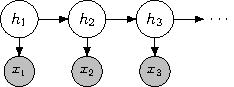
\includegraphics[width=0.45\columnwidth]{figures/hmm.pdf}
    \label{fig:examples-hmm}
  }
%  \subfigure[Directed grid model] {
%    \label{fig:examples-grid}
%    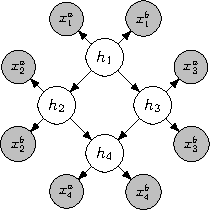
\includegraphics{figures/grid.pdf}
%  }
  \subfigure[Tree model] {
    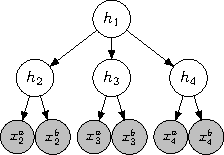
\includegraphics[width=0.45\columnwidth]{figures/tree.pdf}
    \label{fig:examples-tree}
  }
  \subfigure[Noisy-or model] {
    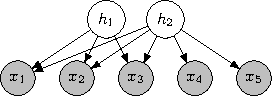
\includegraphics[height=5em]{figures/non-example.pdf}
    \label{fig:examples-noisy-or}
  }
  \caption{(a) and (b): graphs that satisfy the exclusive views property; (c) does not.}
  \label{fig:examples}
\end{figure}


\paragraph{Example: hidden Markov model.}

In the HMM (\figureref{examples-hmm}), the parameters
are $O \eqdef \Pr(x_i|h_i)$ and $T \eqdef \Pr(h_{i+1} | h_i)$
for all $i$. % (i.e. we have parameter sharing).
While the first and last hidden variables $h_1, h_M$ in the
  sequence are not bottlenecks, they still have exclusive views ($x_1$ and
  $x_M$, respectively)
  due to parameter sharing.
  %whose parameters we know because they share parameters, $O$.
%We first use the bottleneck $h_2$ with views $x_1, x_2, x_3$ to estimate $O$,
%and then recover $\pi$ from $\{h_1\}$ and recover $T$ from the clique $\{h_{1}, h_{2}\}$.

\paragraph{Example: latent tree model.}

In the latent tree model (\figureref{examples-tree}), the parameters
are $\pi \eqdef \Pr(h_i)$, $T \eqdef \Pr(h_i | h_1)$ for $i \in \{2,3,4\}$,
and $O \eqdef \Pr(x^a_i | h_i) = \Pr(x^b_i | h_i)$ for $i \in \{2,3,4\}$.
Note that while $h_1$ is not directly connected to an observed variable,
  it is still a bottleneck, with views $x^a_2, x^a_3, x^a_4$.
We can recover $T$ from the clique $\{h_1, h_2\}$ by using views $x^a_2$
  (exclusive to $h_2$) and $x^a_3$ (exclusive to $h_1$).
  %Note that while
  %$x^a_3$ is also a view for $h_2$, $x^a_3$ is independent of $h_2$ given
  %$h_1$.

%In step 1, we recover the parameters $O$ from the bottleneck $h_2$ with
%  views $\{x^a_2, x^b_2, x^a_3\}$. We also recover the conditional moments
%  $\mOpp{2}{1}$, $\mOpp{3}{1}$, $\mOpp{4}{1}$ for $h_1$. 
%In step 2, we can recover $\pi$ from the clique $\{h_1\}$, using any
%  one of views (they are all exclusive). 
%To recover $T$ from the clique $\{h_1, h_2\}$, we use the views $x^a_2$
%  (exclusive to $h_2$) and $x^a_3$ (exclusive to $h_3$). Note that while
%  $x^a_3$ is also a view for $h_2$, $x^a_3$ is independent of $h_2$ given
%  $h_1$.

\paragraph{Non-examples}
\label{sec:non-example}

%In a certain sense, having three views is necessary for identifiability;
%two views is certainly not enough.
% PL: perhaps too simple, saving space
%The simplest example of a model that cannot be recovered by our algorithm is
%  a mixture model with a single view, i.e. \figureref{three-view} with
%  just the variables $h_1$ and $x_1$.
%However, without further assumptions the model itself is not
%  identifiable\footnote{To see this, observe that probability-mass
%  can be arbitrarily exchanged between $\Pr(h_1)$ and $\Pr(x_1 | h_1)$ while preserving the marginals $\Pr(x_1)$}.
%A class of binary-valued noisy-or networks
%(see \figureref{examples-noisy-or} for an example)
%which do not possess the
%  bottleneck property are nonetheless identifiable;
%  see \citet{halpern13noisyor} for an algorithm.
%Having three views is in some sense necessary for the uniqueness of tensor factorization.
There are certainly models which are identifiable but do not have exclusive views.
For example, \figureref{examples-noisy-or} shows
  a binary-valued noisy-or network which can be
  learned by the algorithm of \citet{halpern13noisyor},
  but does not satisfy the exclusive views property.

%%%%%%%%%%%%%%%%%%%%%%%%%%%%%%
\subsection{Sample complexity}
\label{sec:sampleComplexity}
% PL: "combine" is too vague to be useful
%\LearnMarginals combines two consistent algorithms, \TensorFactorize and
%\LearnCliqueNs, and is thus consistent itself.

%In this section, we provide formal conditions under which $\LearnMarginals$
%will produce consistent estimates.
%We let
%$\mOpphat{v}{i}$,
%$\hat Z_\sC$,
%and $\hat M_\sV$,
%denote estimators for
%$\mOpp{v}{i}$,
%$Z_\sC$,
%and $M_\sV$,
%respectively.

% But $\mOpp{v}{i}$ is a product of tensors on the path from $h_i$ to
%   $x_v$, marginalizing out the rest of the graph.
% To make this property more interpretable, let us assume the following
%   property which we prove to be sufficient in
%   \appendixref{assumption-proof}:
% \begin{assumption} 
% \label{asm:full-rank-plus}
% The marginal distribution of every latent variable has full support:
%   $\forall{h_i \in H},~ \mPi{i} \succ 0$.
% For every clique $\sC \in \sG$ (including ones with observed variables),
%   and every conditional distribution $\Pr(h_c \given \Pa(h_c))$, where
%   $h_c \in \sC$, every {\em tensor unfolding} has full column rank, $k$.
% \end{assumption}
% In our directed grid example (\sectionref{directedExample}), for the
%   clique $\sC = \{ h_1, h_2 \}$ this condition implies $\pi = \Pr(h_1)
%   \succ 0$ and $T = \Pr(h_2 \mid h_1)$ has column rank $k$; for the clique
%   $\sC = \{ h_1, x_1 \}$, it implies $O = \Pr(x_1 \mid h_1)$ has column
%   rank $k$.

%\todo{did they prove this; if so just say "they show", not "we can show"}
%Using results from
%  \citet{anandkumar12moments,anandkumar13tensor} we can show that
%  learning $\mOpp{v_1}{i}$ for the bottleneck $h_i$ with views $x_{v_1},
%  x_{v_2}, x_{v_3}$ has the following sample complexity,
%  \todo{define hat O}
%  \todo{max subscript is misaligned}
%\begin{align*}
%  \|\mOpphat{v_1}{i} - \mOpp{v_1}{i}\|^2_F &= \frac{1}{\sqrt{n}} O\left( \frac{k {\pi\oft{i}}_{\max}^2}{\sigma_k(M_{v_1,v_2})^5} \right). 
%\end{align*}
It is easy to see that $\LearnMarginals$ has a polynomial sample complexity because it composes two parts that individually have polynomial sample complexity.
From \citet{anandkumar13tensor} given the non-degeneracy assumptions
  \assumptionref{non-degeneracy}, we have that $\mOpphat{v}{i}$
  converges to $\mOpp{v}{i}$ at a rate of $n^{-\frac12}$ with a constant
  that depends polynomially on the $k$-th singular value of
  $\mOpp{v}{i}$.
% PL: we don't have a crisp theorem (because there's multiple paths), so leave it vague.
Recovering the marginals $Z_\sC$ from the conditional moments via $\LearnClique$ is a linear operation and thus also has polynomial sample complexity. 
Note that $\sigma_{k}(\mOpp{v}{i})$ can become extremely
small if $h_i$ and $x_v$ are connected via many intermediate hidden variables.
\todo{cite work - Sontag?}
%\begin{theorem}[Sample complexity for $\mOpp{v}{i}$]
%  \label{thm:sample-complexity}
%  Without loss of generality, let $v=1, i=1$, and let $x_1, x_2, x_3$ be three views for
%  $h_1$. With probability at least $1 - \delta$,
%\begin{align*}
%  \|\mOpphat{1}{1} - \mOpp{1}{1}\|_F 
%    &\le  \\
%    &
%  \hspace{-0.3in}
%      O\left(
%      % PL: remove pi_max because that's upper bounded by 1.
%      \frac{k \log(1/\delta) } 
%      {\sqrt{n} \, \pi\oft{1}_{\min} (\sigma_{k}(\mOpp{1}{1}) \sigma_{k}(\mOpp{1}{2}))^{5/2}} \right),
%\end{align*}
%where $\pi\oft{1}_{\min}$ is the smallest element of $\pi\oft{1}$.

%If $\sigma_{\min}(\Pr(c \given \Pa(h_c))) \le \sigma$ for every clique
%  $\sC \in \sG$ and hidden variable $h_c \in \sC$,
%\begin{align*}
%  \|\mOpphat{1}{1} - \mOpp{1}{1}\|_F 
%    &\le 
%      O\left( 
%      \frac{k \log(1/\delta) {\pi\oft{1}}_{\max}/{\pi\oft{1}}_{\min}} 
%      {\sqrt{n} \sigma^{5t}} \right) \epsilon,
%\end{align*}
%where $t$ is the length of the shortest topological ordering from $h_1$
%to the unique parent of $x_1$, $h_t$.
%\end{theorem}
%In general, $\sigma_{k}(\mOpp{v}{i})$ will depend exponentially on the
  %path length between the hidden variable $h_i$ and $x_v$.
%This is expected because the influence from $h_i$ to $x_v$
  %gets diluted for every latent variable it must factor through.

%\theoremref{sample-complexity}, proved in \appendixref{assumption-proof}
%  says that the number of samples required to estimate the view
%  $\mOpp{v}{i}$ grows exponentially in the {\em distance} between $x_v$
%  and $h_i$. 

%\todo{Present sample complexity bounds for $Z_\sC$?}

% Easy case
% Next, we need to show that the hidden marginals $\hat Z_\sC$ converge to $Z_\sC$.
% First, $\hat M_\sV$ is just an empirical average of multinomials over the data points.
% Abusing notation slightly, we let $\hat M_\sV$ also denote its
% $d^{m}$-dimensional vectorized version.
% We also represent $\mH_\sC$ as
%   a vector in $\Re^{k^m}$, and represent $\mOppAll \eqdef
%   \mOpp{v_1}{i_1} \otimes \cdots \otimes
%   \mOpp{v_m}{i_m}$ as a matrix in $\Re^{d^m \times
%   k^m}$.
% By the central limit theorem, we have:
% $\sqrt{n} (\hat M_\sV - M_\sV) \convind \sN(0, \Sigma_\sV)$,
% where $\Sigma_\sV$ is the \emph{asymptotic variance} of $\hat M_\sV$: 
% % ARUN: I don't think so - \todo{doesn't this need to be multiplied by something?}
% \begin{align*}
% \Sigma_\sV \eqdef \dM_\sV - M_\sV M_\sV^\top, \quad \dM_\sV \eqdef \text{diag}(M_\sV).
% \end{align*}
% 
% Our next step will be to use the delta-method to convert the above
% result into the asymptotic variance for the pseudoinverse version of
% $\LearnClique$. 
% \begin{lemma}[Asymptotic variance of pseudoinverse estimator for $\tilde Z_\sC$]
%   \label{lem:mom-variance}  
%   Assume $\hat M_{\sV}$ has asymptotic variance $\Sigma_\sV$ defined above.
%   Then the asymptotic variance of $\hat{Z_\sC}$ is:
%   \begin{align*}
%     \Sigma^{\mom} &= \mOppAlli \Sigma_\sV \mOppAllit.
%   \end{align*}
%   %where ${\mOppAll}\pinv \eqdef {\mOpp{v_1}{i_1}}\pinv \otimes
%   %\cdots \otimes {\mOpp{v_m}{i_m}}\pinv$, a $d^m \times k^m$ matrix.
% \end{lemma}
% \begin{proof}
% For clique $\sC$, recall we have
%   $Z_{\sC} = \mO_\sV(\mOppi{v_1}{i_1},\cdots,\mOppi{v_m}{i_m})$.
% %Choosing to represent $Z_\sC$ and $M_\sV$ as vectors and
% %$\mOppi{v_1}{i_1} \otimes \cdots \otimes \mOppi{v_m}{i_m}$ as the
% %matrix,
% We can rewrite this representation more compactly as: $Z_{\sC} = {\mOppAll}\pinv \mO_\sV$.
% By the delta-method \cite{vaart98asymptotic},
% % DONE: need to shorten
% %we have that the asymptotic variance of $M_\sV$ is:
% %\begin{align*}
% %  \sqrt{n}(\hat M_\sV - M_\sV) \convind \sN(0, \Sigma_\sV),
% %\end{align*}
% %where $\Sigma_\sV$ is the variance of the observations. 
% we immediately get:
% $\sqrt{n}(\hat Z_\sC - Z_\sC) \convind \sN(0, \mOppAlli \Sigma_\sV \mOppAllit)$.
% \end{proof}

% DONE: too brazen to say
%Note that extending these results to finite sample bounds can be done
  %via a straightforward application of perturbation bounds.
